\documentclass[chaptersright]{informeutn}
\usepackage[utf8]{inputenc}
\usepackage{array}
\usepackage{geometry}
\usepackage[table]{xcolor}
\usepackage{colortbl}
\usepackage{caption}

\materia{Dispositivos Electronicos I}
\titulo{Trabajo Practico N°2: Diodos rectificadores y zener}
\comision{3R2}
\autores{Documentador y operador: Gaston Grasso 401892\\ Coordinador: Angelo Prieto 401012}
\fecha{27-05-2025}

\begin{document}
\maketitle
\tableofcontents

\chapter{Introduccion}

  En este segundo trabajo práctico se analizó y midió el comportamiento de diodos rectificadores, tanto de silicio como 
  de germanio, y de diodos zener. Se busca:
  
  \begin{itemize}
    \item Entender su funcionamiento.
    \item Comparar el diodo ideal simulado con el diodo real.
    \item Ver como la curva es afectada por la temperatura del dispositivo.
  \end{itemize}


\chapter{Identificacion de pines}

  \begin{center}
  \begin{table}[h!]
  \centering
  \renewcommand{\arraystretch}{2}
  \begin{tabular}{|m{4cm}|>{\centering}m{2cm}|>{\centering}m{2cm}|>{\centering}m{2cm}|>{\centering\arraybackslash}m{2cm}|}
  \hline
  \textbf{Sentido de las puntas del multímetro} & \multicolumn{2}{c|}{\textbf{Diodo de silicio}} & \multicolumn{2}{c|}{\textbf{Diodo de germanio}} \\
  \cline{2-5}
  & D1 & D2 & D1 & D2 \\
  \hline
  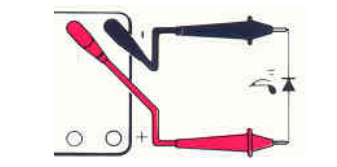
\includegraphics[width=3.5cm]{pictures/polaridad_multimetro1.png} &  &  &  &  \\
  \hline
  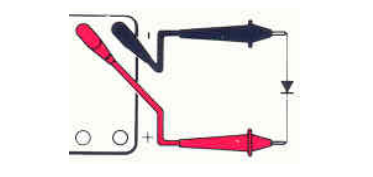
\includegraphics[width=3.5cm]{pictures/polaridad_multimetro2.png} &  &  &  &  \\
  \hline
  \end{tabular}
  \caption{Resultados de las mediciones con el multimetro en modo diodo}
  \end{table}
  \end{center}





\chapter{Curva caracteristica del diodo}

  \section{Actividad de simulación}
  
  \section{Actividad de laboratortio}
  
    \subsection{Diodo de silicio}
    
      \begin{table}[h!]
      \centering
      \renewcommand{\arraystretch}{1.5}
      \setlength{\tabcolsep}{8pt}
      \begin{tabular}{|c|*{13}{c|}}
      \hline
      \textbf{$V_1$ [V]} & 0 & 0.1 & 0.3 & 0.4 & \cellcolor{yellow}0.45 & \cellcolor{yellow}0.5 & \cellcolor{yellow}0.55 & \cellcolor{yellow}0.6 & \cellcolor{yellow}0.65 & \cellcolor{yellow}0.7 & 1 & 3 & 5 \\
      \hline
      $V_D$ &  &  &  &  &  &  &  &  &  &  &  &  &  \\
      \hline
      $I_D$ &  &  &  &  &  &  &  &  &  &  &  &  &  \\
      \hline
      \end{tabular}
      \caption{Tabla de valores $V_D$ e $I_D$ para diodo de silicio 1N4007.}
      \label{a}
      \end{table}
    
    \subsection{Diodo de germanio}
    
      \begin{table}[h!]
      \centering
      \renewcommand{\arraystretch}{1.5}
      \setlength{\tabcolsep}{8pt}
      \begin{tabular}{|c|*{13}{c|}}
      \hline
      \textbf{$V_1$ [V]} & 0 & 0.1 & 0.3 & 0.4 & \cellcolor{yellow}0.45 & \cellcolor{yellow}0.5 & \cellcolor{yellow}0.55 & \cellcolor{yellow}0.6 & \cellcolor{yellow}0.65 & \cellcolor{yellow}0.7 & 1 & 3 & 5 \\
      \hline
      $V_D$ &  &  &  &  &  &  &  &  &  &  &  &  &  \\
      \hline
      $I_D$ &  &  &  &  &  &  &  &  &  &  &  &  &  \\
      \hline
      \end{tabular}
      \caption{Tabla de valores $V_D$ e $I_D$ para diodo de germanio 1N60.}
      \label{b}
      \end{table}

\chapter{Comportamiento del diodo en funcion de la temperatura}

\chapter{Circuitos recortadores con diodos zener}

  \section{Actividad de simulación}
  
  \section{Actividad de laboratortio}

\chapter{Análisis sobre parámetros de hoja de datos}

  \section*{Características Eléctricas}
  
    \subsection*{Regímenes máximos}
      \begin{enumerate}
        \item $V_{RRM}$: Tensión repetitiva máxima en inversa. Es el máximo voltaje que se puede aplicar en polarización inversa de manera repetitiva sin dañar el dispositivo.
        \item $V_{RSM}$: Tensión máxima en inversa no repetitiva. Es el valor pico máximo que puede soportar el dispositivo en condiciones excepcionales.
        \item $I_{FRMS}$: Corriente eficaz directa máxima. Es la corriente RMS que el dispositivo puede conducir de forma continua sin sobrecalentamiento.
        \item $I_{FSM}$: Corriente de sobrecarga directa máxima. Es el valor pico máximo de corriente directa que puede soportar durante un pulso corto.
      \end{enumerate}
    
    \subsection*{Regímenes característicos}
      \begin{enumerate}
        \item $V_{BR}$: Tensión de ruptura. Es el voltaje en el cual el dispositivo comienza a conducir en inversa.
        \item $I_R$: Corriente de fuga inversa. Es la pequeña corriente que circula en inversa antes de la ruptura.
        \item $V_F$: Tensión de conducción directa. Es la caída de tensión directa cuando el dispositivo está conduciendo.
        \item $I_{RM}$: Corriente máxima en inversa. Es la máxima corriente que puede circular en polarización inversa antes de entrar en ruptura.
        \item $I_F$: Corriente directa. Es la corriente que circula a través del dispositivo cuando está polarizado en directa.
      \end{enumerate}
  
  \section*{Características Térmicas}
  
    \begin{enumerate}
        \item $T_J$: Temperatura de unión máxima. Es la temperatura máxima permitida en la unión del semiconductor durante su operación.
        \item $T_{STG}$: Temperatura de almacenamiento. Es el rango de temperatura dentro del cual se puede almacenar el dispositivo sin que sufra daños.
        \item $T_A$: Temperatura ambiente. Es la temperatura del entorno en el cual opera el dispositivo.
        \item $R_{\theta jc}$: Resistencia térmica unión-carcasa. Indica la resistencia al flujo de calor desde la unión interna del dispositivo hasta su encapsulado.
    \end{enumerate}
  
  \section*{Características de uso}
  
    \begin{enumerate}
        \item $V_{RMS}$: Tensión eficaz. Es el valor eficaz de la tensión alterna aplicada al dispositivo.
        \item $P_{tot}$: Potencia total disipada. Es la máxima potencia que el dispositivo puede disipar sin exceder los límites térmicos.
        \item $T_r$: Tiempo de recuperación. Es el tiempo que tarda el dispositivo en dejar de conducir una vez que se retira la señal de conducción.
    \end{enumerate}

\chapter{Conclusión final}
\end{document}
